\documentclass[10pt]{article}              % Book class in 11 points
\parindent0pt  \parskip10pt             % make block paragraphs
\usepackage[dvips]{color}

\usepackage{tcolorbox}
\tcbuselibrary{breakable}

\usepackage{afterpage}

\usepackage{xcolor}
\usepackage[basque]{babel}
\selectlanguage{basque}
\usepackage[hmargin=2.5cm,vmargin=2.5cm,headheight=15pt]{geometry}
\usepackage{graphicx}
\usepackage{amsmath,amsfonts,amssymb}
\usepackage{mathrsfs}  

%\usepackage{picins}

\begin{document}                        % End of preamble, start of text.




\section*{2018-2019 Ikasturtea, 
\textit{Termodinamika eta Fisika Estatistikoa}\\
Ez-ohiko deialdia, 
2019ko ekainaren 25a}

%\vspace{0.25cm}
%%%%%%%%%%%%%%%%%%%%%%%%%%%%%%%%%%%%%%%% termodinamika
\section*{Termodinamika}

\begin{enumerate}

\item Erantzun itzazu laburki eta arrozonatuz:

\begin{enumerate}
%\item Lortu $H$, $U = \frac{{AS^3 }}{{27NV}}$ oinarrizko ekuaziotik abiatuz.
\item Ondorioztatu ondoko adierazpena:

$H =  - T^2 \left( {\frac{{\partial \left( {{G \mathord{\left/
 {\vphantom {G T}} \right.
 \kern-\nulldelimiterspace} T}} \right)}}{{\partial T}}} \right)_p$

\item Esku artean dugun sistemari esleitu zaion egoera-ekuazioa ondoko itxurakoa da: $V = R\frac{T}{p} - \frac{C}{{T^2 }}$, non $R$ eta $C$ konstanteak diren. Lortu prozesu isotermoetako entropia-aldaketa eta entalpia-aldaketa.
\item Lortu $C_v  = A + BT$ bero-ahalmeneko gas ideal poliatomikoari dagokion lerro adiabatiko itzulgarrien adierazpena. $A$ eta $B$ konstanteak dira.
%\item Frogatu $\mu$ potentzial kimikoa masa unitateko $G$ potentzial termodinamikoa dela.
\item Demagun esku artean sistema hidrostatikoa dugula. Zeren berdina da entalpia-aldaketa, presio konstanteko prozesuan? (Beste modu batean, zer neurtuko du entalpia-aldaketak aipatu prozesuan?)
%\item Ondokoa da aztergai dugun sistemari dagokion $\alpha$ zabalkuntza-koefizientearen adierazpena:
%
%\begin{center}
%$\alpha  = \frac{{f(p)}}{T}$
%\end{center}
% 
%Nolakoa da $C_{p}$ koefizienteak presioarekiko duen mendekotasuna?
\end{enumerate}

\item[]

%%%%

\item Irudian ageri den zilindroaren alboko hormak adiabatikoak, iragaztezinak eta ez-higikorrak dira, goikoa eta behekoa aldiz, higiezinak, iragaztezinak eta diatermoak. Zilindroaren erdian kokatu den pistoi adiabatikoak, iragaztezinak eta higikorrak $V_{0}$ bolumeneko bi gunetan zatitu du zilindroa. Goiko gunean, $c_{V}$ bero-ahalmeneko gas ideal baten $n=\frac{1}{R}$ mol dago. Beheko gunean, lurruna eta likidoaren arteko orekan dagoen sistemaren 3 mol dago; sistema horren moleko lurruntze bero-sorra $l$ da, $T_{0}$ eta $p_{0}$ direnean. Gainera, fase kondentsatuak bete duen bolumena $\frac{V_{0}}{2}$ da. Beheko gunean dagoen sistemaren bolumenen arteko erlazioa hauxe da: $2v_{l}=v_{g}$. Beheko zilindroaren eta $\frac{T_{0}}{2}$ tenperatura dagoen bero-iturriaren artean \textit{Carnot}-en makina bat kokatu da; horrek sistematik beroa ateratzen du, jakinik sistema faseen arteko orekan beti dagoela. Azkenik, makinak ateratako lana oso-osorik bero moduan era kuasiestikoan ematen zaio goiko guneari. Prozesua bukatutzat emango da lurruna desagertu denean.

Lor itzazu honako hauek:
\begin{enumerate}
\item gas idealaren bukaerako tenperatura,
\item bero-iturri hotzari emandako bero kantitatea, eta
\item gas idealaren eta sistemaren entropia-aldaketak.
\end{enumerate}

\end{enumerate}

\begin{center}
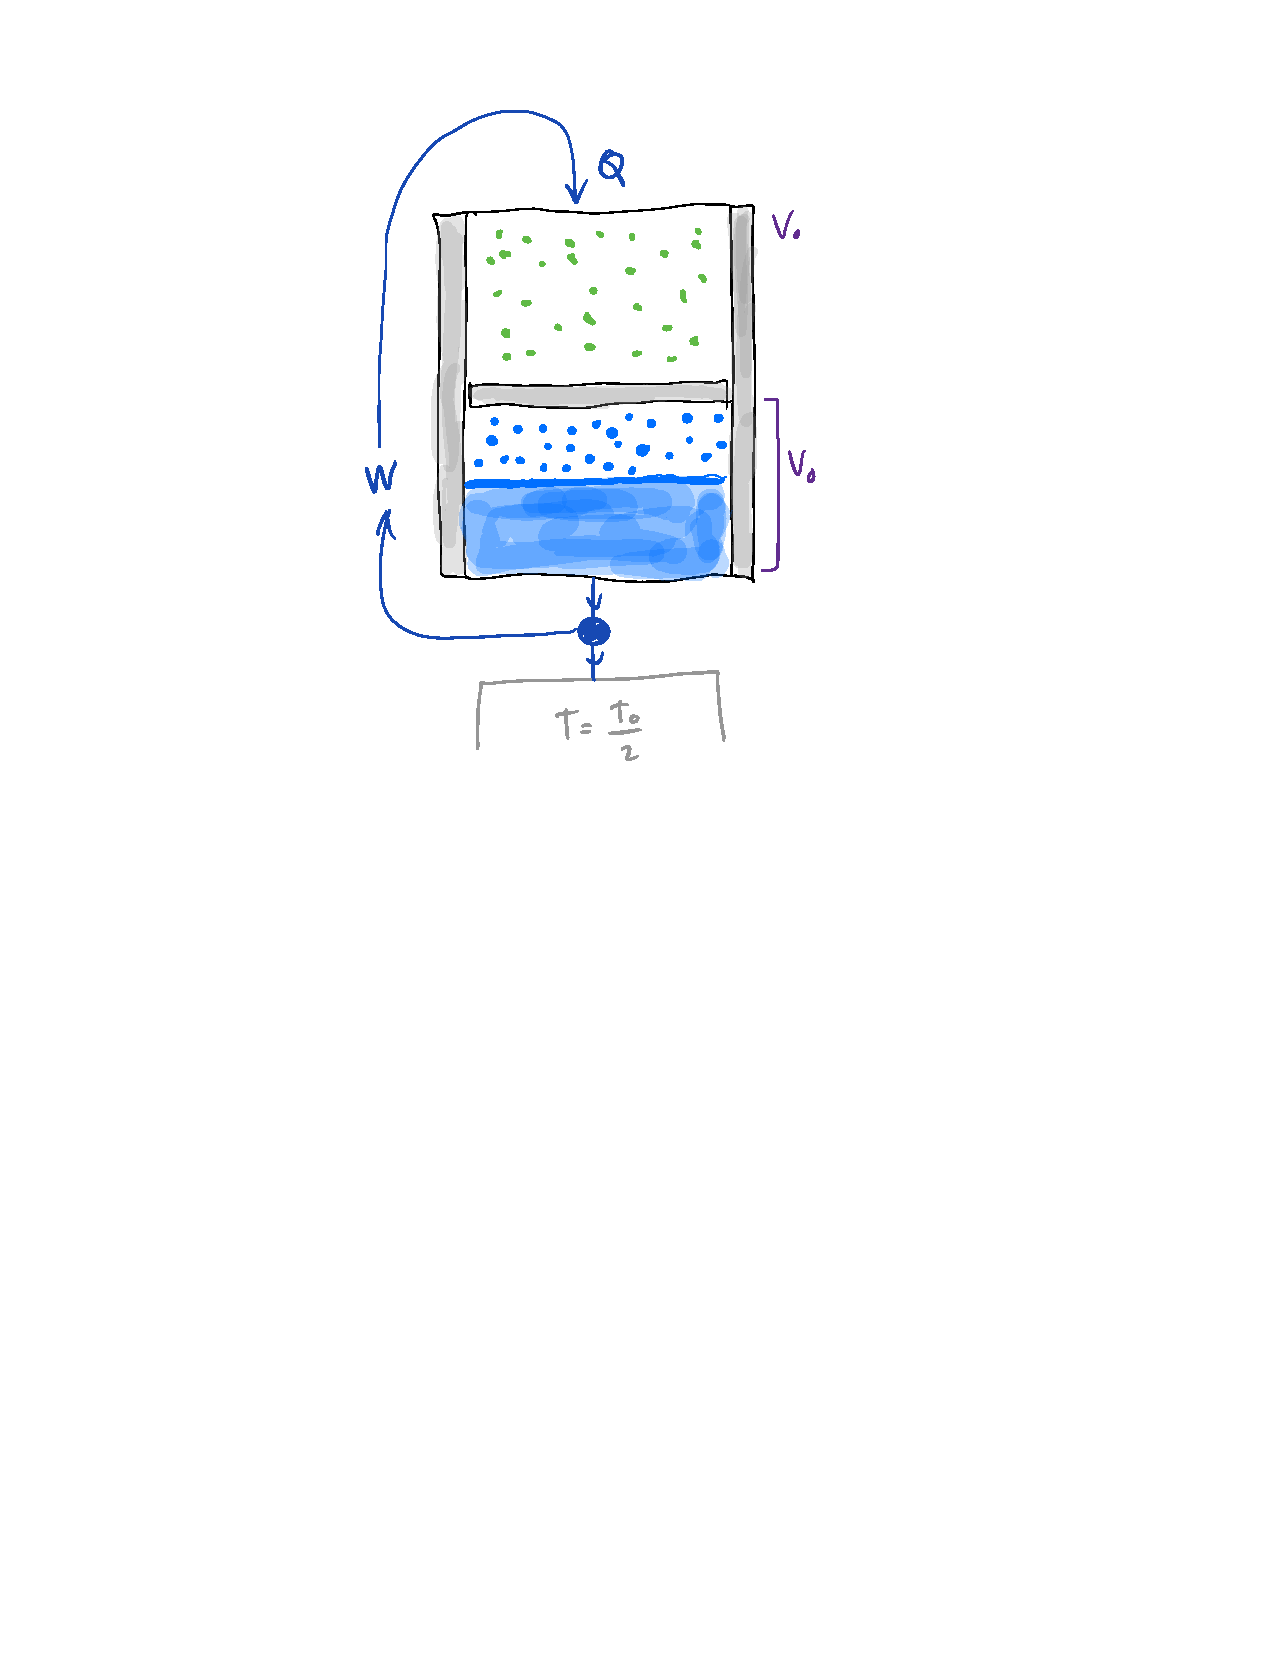
\includegraphics[width=5.6cm]{11PAzterketaPartzialaIrudia.pdf}
\end{center}


%%%%%%%%%%%%%%%%%%%%%%%%% ESTATISTIKA
%---------------------------------------
% 1a ariketa
\cleardoublepage

\section*{Estatistika}

\begin{enumerate}

\item[] \textbf{$\epsilon(\textbf{p}) = \alpha\,|\textbf{p}|^{3(\gamma - 1)}$ dipertsio-erlazioko gasa}
\vspace{0.25cm}

\item Aztertu behar duzun gasaren partikula osatzaile independenteen energia zinetikoa honako hau da: $\epsilon(\textbf{p}) = \alpha\,|\textbf{p}|^{3(\gamma - 1)}$. Adierazpen horretan $\alpha$ da konstante bat; $\textbf{p}$ da momentua, $L^{3}$ bolumeneko kutxan honako era honetan kuantizatutakoa bera: $p_{x}=\frac{h\,n_{x}}{L}$, $p_{y}=\frac{h\,n_{y}}{L}$ eta $p_{z}=\frac{h\,n_{z}}{L}$ eta $n_{x}$, $n_{y}$ eta $n_{z}$, zenbaki osoak. Horien adibideak dira partikula ez-erlatibistak eta partikula ultra-erlatibistak, zeintzuen kasuan $\gamma = \frac{5}{3}$ eta $\gamma=\frac{4}{3}$ diren, hurrenez hurren.

\begin{enumerate}
\item Erabili Multzo Mikrokanonikoa frogatzeko ezen prozesu adiabatikoa batean $p\,V^{\gamma} = \textrm{konstante}$ dela.
\item Lortu aurreko ataletik energia dela: $E = \dfrac{N\,k_{B}\,T}{\left(\gamma -1 \right)}$
\item Lortu lehen ataletik entropia dela: $S = \dfrac{N\,k_{B}}{\left(\gamma -1 \right)}\,\ln\left( pV^{\gamma}\right) + f(N)$
\item Lortu $\dfrac{C_{p}}{C_{V}}=\gamma$
%\item Errepikatu 1 atala Multzo Kanonikoa erabiliz
\end{enumerate}

\vspace{1cm}

\item[]
\item[] \textbf{$T=0$ K tenperaturako e$^{-}$ propietate magnetikoak}


\item Elektroiak aztertuko dituzu, $T=0$ K tenperaturan dagoen kutxan sartutako $m$ masako eta $\frac{1}{2}$ spineko elektroiak hain zuzen. Kutxa ezarri da $B$ eremu magnetikoaren pean eta, ondorioz, elektroiek harekin duten elkarrekintza-energia $-\gamma\,B\,\sigma_{z}$ da; $\gamma$ da erradio giromagnetikoa.\\

Ebatzi segidako bi galderak kutxaren dimentsioak 1, 2 eta 3 direnean eta, ondorioz, kutxaren \textit{bolumena} $L$, $A$ eta $V$ denean

\begin{enumerate}
\item Deskribatu partikula bakarraren egoeren dentsitatea, ezberdinduz \textit{gorako} eta \textit{beherako} spin-egoerak.
\item \textbf{Sailkatu} dimentsioan beheko adierazpide grafikoak eta \textbf{bete} falta diren datuen balioak, hots: $M_{s}$, $B_{c}$ eta $\chi$.
\end{enumerate}

\noindent Horretarako erabili bakarrik $\gamma$, $m$, $N$, $L$, $A$, $V$.


\end{enumerate}

\begin{center}
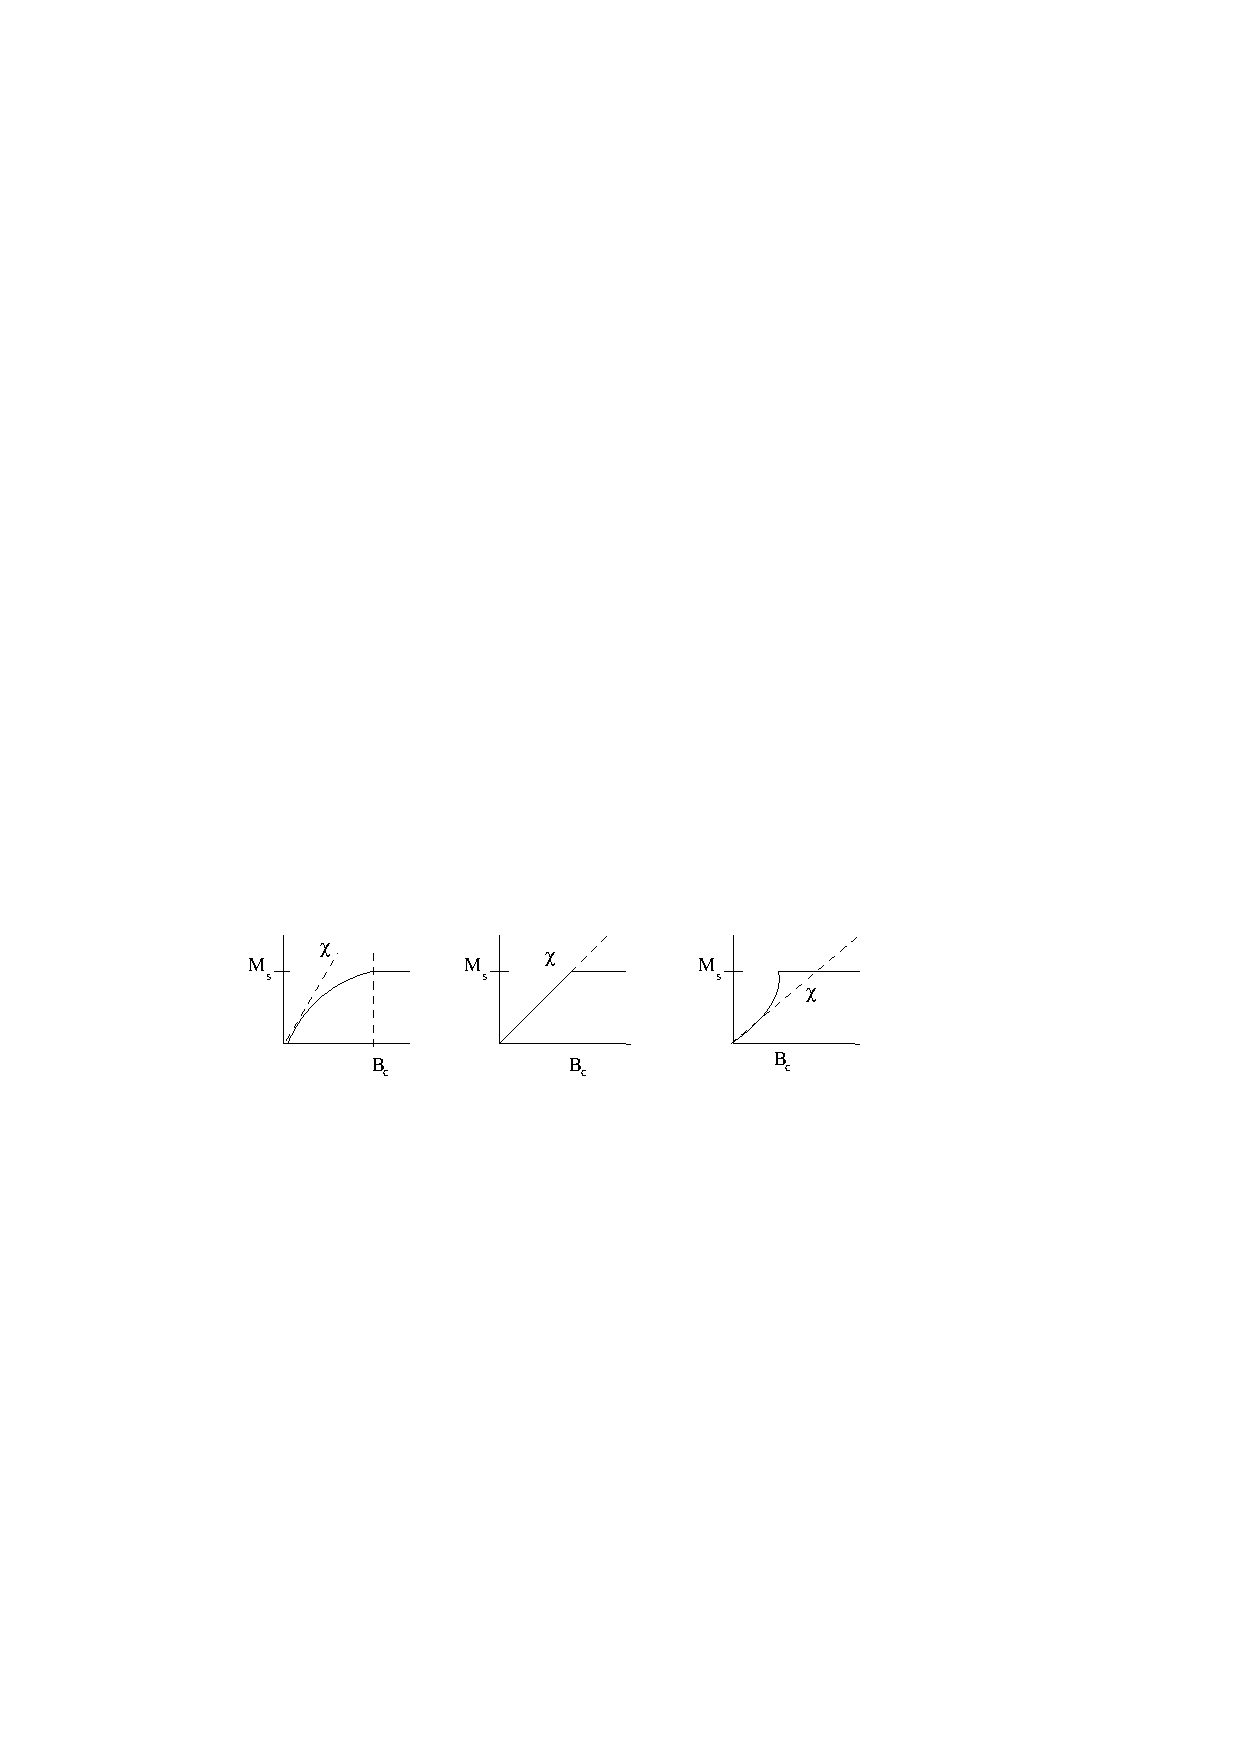
\includegraphics[width=14.2cm]{1PAzterketaPartzialaIrudia.pdf}
\end{center}




\end{document}

